% !TeX spellcheck = en_GB
\chapter{Implementation and Testing} % Realisierung und Test
\epigraph{Any fool can write code that a computer can understand. Good programmers write code that humans can understand.}{Martin Fowler}


\section{Development Setup}

Figure \fullref{fig:development-setup} illustrates the development setup in the form of an UML deployment diagram.
A developer connects via his browser to the reverse proxy that serves the XMPP-Grid Broker web application.
The HTTP-Connection from the client to the server is secured using TLS-mutual authentication.
The same reverse proxy also routes the XMPP connections.
The client also authenticates to the proxy using TLS-mutual authentication, and the proxy afterwards establishes a TLS connection to the XMPP server using his client certificates.
The reasons for this setup is described in more detail in \fullref{todo}.

\begin{figure}[h]
    \centering
    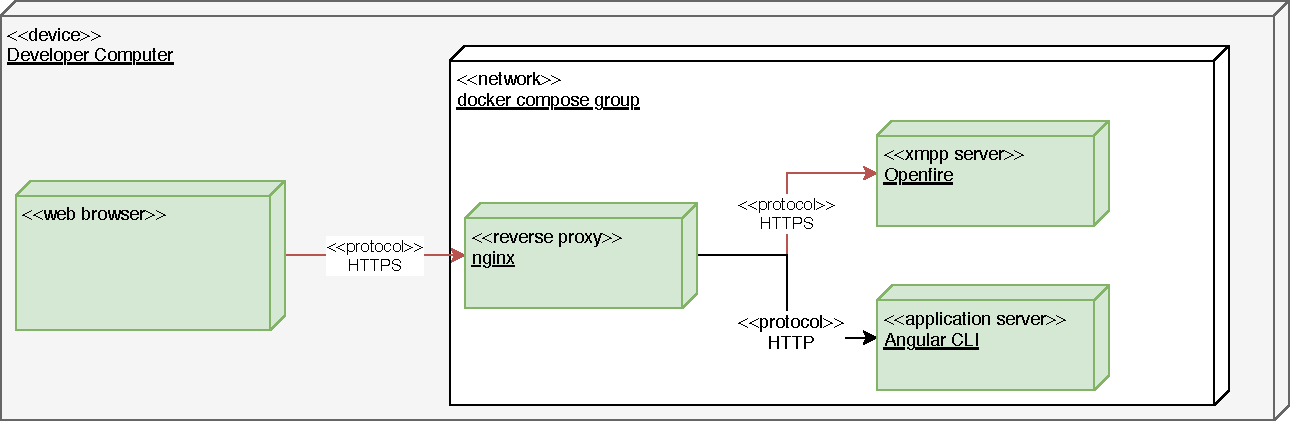
\includegraphics[width=1\linewidth]{resources/development-setup-uml}
    \caption{UML Deployment Diagram presenting the development setup}
    \label{fig:development-setup}
\end{figure}

As the previously described structure is not trivial, the guiding principle for our development setup was to maximise automation and minimise manual setup and configuration efforts as this is the basis for a durable software.
We decided on a docker and docker-compose based stack that provides a correctly setup Openfire instance, a preconfigured nginx instance as well as client and server certificates.
Everyday tasks such as generating new certificates or building and testing the application and documentation were automated in bash scripts.

The efforts invested in this docker setup also paid off when we began to write integration tests that run in the same environment.

We deliberately decided to run unit test outside of the docker environment as unit tests are executed more often, and the additional docker-overhead would, therefore, be unnecessarily expensive.
Also, debugging is more straightforward without any indirections.

\section{Encountered Problems}

\subsection{Limitations of \emph{\fullref{sec:requirement-multiple-administrators}}}\label{sec:limitations-of-requirement-multiple-administrators}

Requirement \ref{sec:requirement-multiple-administrators} states that multiple administrators should be able to access the application.

When authenticating users with SASL EXTERNAL, the client certificate extension field `xmppAddr' is interpreted as user \gls{jid} by the \gls{xmpp} server.

In practice, most \gls{xmpp-grid} \gls{broker} deployments will require an HTTP proxy in front of the \gls{xmpp} server as security measure\footnote{
More information on this can be found in Section~\fullref{sec:implemented-web-application-topology}.}.
Usually, the HTTP proxy can also be used to serve the \gls{broker} application.
Such an HTTP proxy might also accept multiple different client certificates.

If the client connects to the \gls{xmpp} server over secure WebSockets (WSS) in combination with SASL EXTERNAL, the WebSocket URL must already be authenticated, as most browsers do not permit certificate selection on background requests\footnote{\url{https://bugs.chromium.org/p/chromium/issues/detail?id=329884\#c24}}.
This might be achieved by serving the \gls{broker} from the same domain or by using client certificate policies\footnote{\url{https://support.google.com/chrome/a/answer/6080885?hl=en\#manage-certs}}.

As the proxy intercepts the TLS connection, it must verify the client certificate sent by the browser and establish a connection to the \gls{xmpp} server using a client certificate as well.
Therefore, the `xmppAddr' field of the proxy's client ceritifcate is used by the \gls{xmpp} server.
If multiple users should be differentiated on the \gls{xmpp} server, an HTTP proxy might choose different client certificates for connecting to the \gls{xmpp} server based on the web browser's client certificate `xmppAddr'.


\subsection{Limitations of \emph{\fullref{sec:requirement-audit-trail}}}

Actions of administrators should be traceable with an audit trail according to requirement \ref{sec:requirement-audit-trail}.

As outlined in Section~\ref{sec:limitations-of-requirement-multiple-administrators}, practical deployments of \gls{xmpp-grid} \glspl{broker} will mostly use a HTTP proxy.
Additionally, to handling the client authentication, the proxy can be used to keep an audit trail of client requests.
These requests can then be correlated with the query log on the \gls{xmpp} server.

Creating audit trails on the client side does not provide additional safety, as users might prevent trail entries by manipulating the client application.
Therefore, no such mechanism was implemented.


% - Logout (TLS)
% - Initial Topic Consumers and Providers + Initial Topic Consumers and Providers => 2 Step Process!
% - Openfire:
%   - Lost updates with OpenFire
%   - falsche Felder - speziell pubsub#node_type
%   - vgl. https://discourse.igniterealtime.org/t/wrong-field-type-of-pubsub-node-type-and-how-to-update-it/81596
% -> Fehlende Methoden/Funktionalität im Standard
%   - "Liste alle Topics" -> Geht nur hierarchisch
%   - Filtering von Persisted Items

\section{Code Quality}
% - Qualität des Codes
    % - Metriken
    % - Coding Guidelines
    % - Coding Reviews Richtlinien
    % - JavaDoc etc
    % - Patterns
    % - Code stimmt mit Arch. überein

% Typescript mit liter (tslint)
% Best-Practices von Angular befolgt dank Intellij Ultimate (`@angular/language-service`) und https://github.com/mgechev/codelyzer (ink. tslint)
% Modular und Testbar
% Doku mit Compodoc

\subsection{Complexity}
% - Komplexität und Umfang
    % - Metriken

    % Sadly, there are no tools that do this..

\section{Testing}
% - Test
    % - Sinnvoll
    % - Abdeckung der Anforderungen
    % - Coverage
    % - Protokolle

% Viele Angular Component Tests -> Leider grosser gap zwischen test env und realität was testing etwas mühsam macht
% Integration/E2E-Tests mit Protractor
% - mühsam wegen BOSH da immer "polling"

\section{Documentation}
% - Installation
% - Benutzerdokumentation
% - Zielerreichung
% - Architectural Decisions